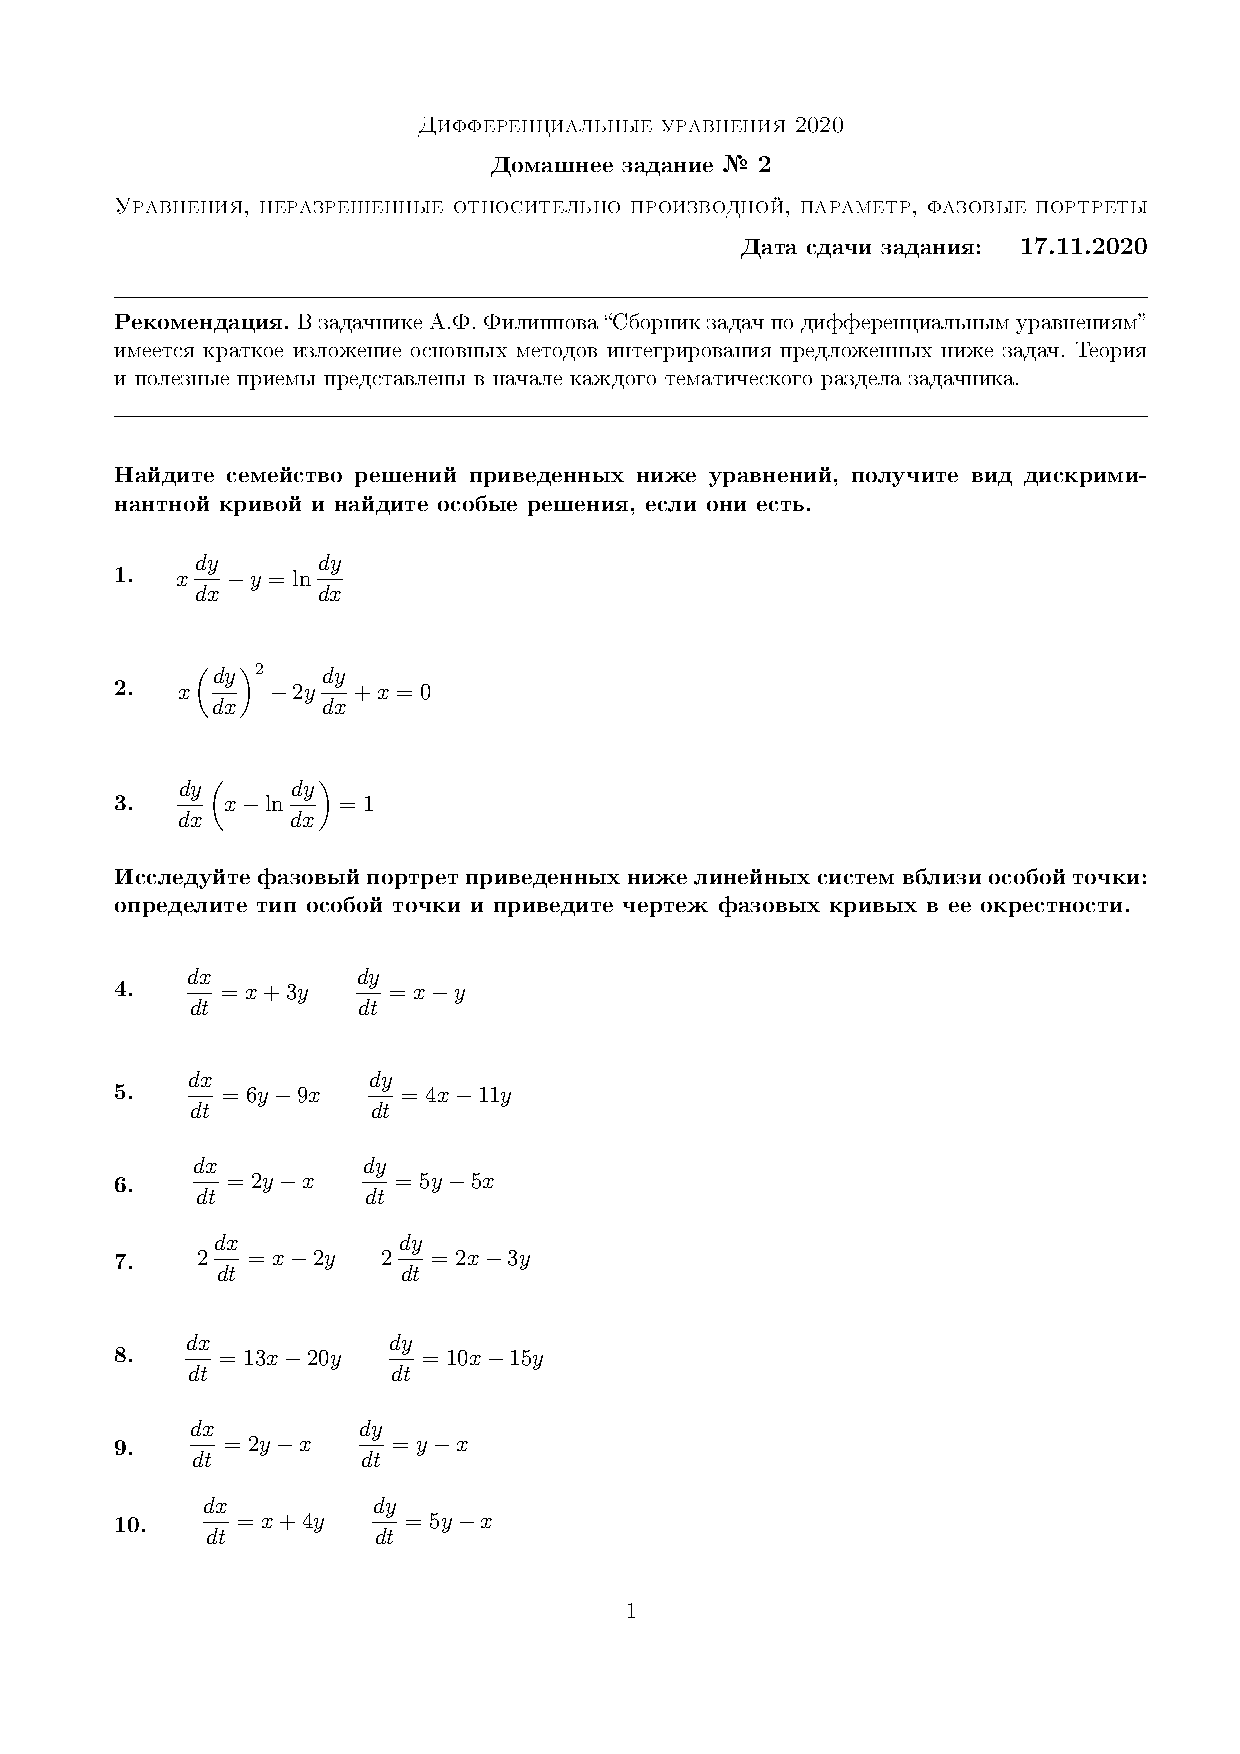
\includepdf[pages=1]{Tasks/HW-2-DE-2020}
\newpage
\section*{Решения}
\subsection*{Задача 1}
	\begin{gather*}
		x \frac{\partial y}{\partial x} - y = \ln \frac{\partial y}{\partial x}\\
		p = y'\\
		y = px - \ln\left(p\right)\\
		\frac{\partial y}{\partial x} = p = p + xp'- \frac{p'}{p}\\
		p'\left(x - \frac{1}{p}\right) = 0\\
		x = \frac{1}{p}\\
		x \frac{1}{x} - y = \ln \frac{1}{x}\\
		y = \ln\left(x\right) + 1
	\end{gather*}
	или
	\begin{gather*}
		p'= 0\\
		p = c\\
		y = xc - \ln\left(c\right)
	\end{gather*}
	Дискриминантные кривые:
	\begin{gather*}
	\begin{cases}
		F = xp - y - \ln\left(p\right) = 0\\
		\frac{\partial F}{\partial p} = x - \frac{1}{p} = 0
	\end{cases}\\
	F = 1 - y + \ln x = 0\\
	y = \ln x + 1
	\end{gather*}
	Особые решения: $y = \ln x + 1$
	\begin{comment}
	\begin{tikzpicture}
		\begin{axis}[
		grid=both,
		minor tick num=4,
		grid style={line width=.1pt, draw=gray!10},
		major grid style={line width=.2pt,draw=gray!50},
		axis lines=middle,
		enlargelimits={abs=0.2},
		xlabel=$x$,
		ylabel={$\ln\left(x\right) + 1$}
		] 
		\addplot[domain=-1:5,samples=1000,smooth,blue]{ln\left(x\right) + 1};
		\end{axis}
	\end{tikzpicture}
	\end{comment}


\newpage
\subsection*{Задача 2}
	\begin{gather*}
		x \left(\frac{\partial y}{\partial x}\right)^2 - 2y \frac{\partial y}{\partial x} + x = 0\\
		p = y'\\
		xp^2 - 2yp + x = 0\\
		D - 4\left(y^2 - x^2\right) \geqslant 0
		y^2 - x^2 \geqslant 0\\
		y = \frac{xp}{2} + \frac{x}{2p}\\
		\frac{\partial y}{\partial x} = p = \frac{p}{2} + \frac{xp'}{2} + \frac{1}{2p} - \frac{xp'}{2p^2}\\
		p\left(1 - \frac{1}{p^2}\right) = xp'\left(1 - \frac{1}{p^2}\right)
	\end{gather*}
	\begin{enumerate}
	\item[$1 - \frac{1}{p^2} = 0$]
		\begin{gather*}
			p = \pm 1\\
			x \pm 2y + x = 0\\
			y = \pm x
		\end{gather*}
	\item[$xp'= p$]
		\begin{gather*}
			p = xc\\
			x^3 c^2 - 2xcy + x = 0\\
			y = \frac{x^2 c}{2} + \frac{1}{2c}\\
			\text{проверим } y^2 - x^2 \geqslant 0\\
			\frac{x^4 c^2}{4} - \frac{x^2}{2} + \frac{1}{4c^2} - x^2 \geqslant 0\\
			x^4 c^2 - 6x^2 + \frac{1}{c^2} \geqslant 0
		\end{gather*}
	\end{enumerate}
	Ответ:
	\begin{gather*}
		y = \pm x\\
		y = \frac{x^2}{c} + \frac{1}{2c}
	\end{gather*}
	Дискриминантные кривые:
	\begin{gather*}
	\begin{cases}
		F = xp^2 - 2yp + x = 0\\
		\frac{\partial F}{\partial p} = 2xp - 2y = 0
	\end{cases}
	p = \frac{y}{x}\\
	F = \frac{y^2}{x} - \frac{2y^2}{x} + x = 0\\
	-\frac{y^2}{x} + x = 0\\
	x^2 = y^2\\
	y = \pm x
	\end{gather*}
	Особые решения: $y = \pm x$
	
	
\newpage	
\subsection*{Задача 3}
	\begin{gather*}
		\frac{\partial y}{\partial x} \left(x - \ln \frac{\partial y}{\partial x}\right) = 1\\
		\frac{\partial y}{\partial x} = p\\
		x = \frac{1}{p} + \ln\left(p\right)\\
		\frac{\partial x}{\partial y} = \left(-\frac{1}{p^2} + \frac{1}{p}\right) \frac{\partial p}{\partial y}\\
		\frac{1}{p} = \frac{p - 1}{p^2} p'\\
		p'= \frac{p}{p-1}\\
		\frac{\partial p}{\partial y} = \frac{p}{p - 1}\\
		\frac{p - 1}{p} \partial p = \partial y\\
		\int \left(1 - \frac{1}{p}\right) \partial p = \int \partial y\\
		p - \ln p = y + c
	\end{gather*}
	Следовательно решение имеет параметрический вид
	\begin{gather*}
	\begin{cases}
		y = p - \ln\left(p\right) + c\\
		x = \frac{1}{p} + \ln\left(p\right)
	\end{cases}
	\end{gather*}
	Дискриминантные кривые
	\begin{gather*}
		\begin{cases}
			F = px - p\ln p -1 = 0\\
			\frac{\partial F}{\partial p} = x - \ln p - 1 = 0
		\end{cases}\\
		\frac{\partial \left(p\ln p\right)}{\partial p} = \ln p + p \frac{1}{p}\\
		\ln p = x - 1\\
		p = e^{x - 1}\\
		F = xe^{x-1} - e^{x-1}\left(x-1\right) -1 = 0\\
		F = e^{x-1} - 1 = 0\\
		x - 1 = 0
	\end{gather*}
	Подставим в исходное уравнение
	\begin{gather*}
		\frac{\partial y}{\partial x} \left(1 - \ln \frac{\partial y}{\partial x}\right) = 1\\
		1 + \ln \frac{\partial x}{\partial y} = \frac{\partial x}{\partial y}
	\end{gather*}
	Так как $x = 1$, то $\frac{\partial x}{\partial y} = 0$, следовательно $x = 1$ не решение и особых решений нет.
	
\newpage
\subsection*{Задача 4}
\begin{figure}[!h]
	\begin{minipage}[h]{0.49\linewidth}
		\begin{gather*}
			\begin{vmatrix}
				1 - \lambda & 3\\
				1 & -1 - \lambda
			\end{vmatrix}
			=
			\lambda^2 - 2\\
			\lambda_1 = 2,\ \lambda_2 = -2
		\end{gather*}
		Найдем собственные вектора
		\begin{gather*}
			\lambda_1 = 2\qquad
			A - \lambda_1 I =
			\begin{pmatrix}
				-1 & 3\\
				1 & -3
			\end{pmatrix}\\
			v_1 =
			\begin{pmatrix}
				3 \\ 1
			\end{pmatrix}
		\end{gather*}
		и
		\begin{gather*}
			\lambda_2 = -2\qquad
			A - \lambda_2 I =
			\begin{pmatrix}
				3 & 3\\
				1 & 1
			\end{pmatrix}\\
			v_2 =
			\begin{pmatrix}
				-1 \\ 1
			\end{pmatrix}
		\end{gather*}
		\begin{gather*}
			T = 
			\begin{pmatrix}
				3 & 1\\
				1 & -1
			\end{pmatrix}\qquad
			T^{-1} = \frac{1}{4}
			\begin{pmatrix}
				1 & 1\\
				1 & -3
			\end{pmatrix}\\
			X = T e^{J t} T^{-1} = \frac{1}{4} e^{2t} 
			\begin{pmatrix}
				3 & 1\\
				1 & -1
			\end{pmatrix}
			\begin{pmatrix}
				1 & 0\\
				0 & -1
			\end{pmatrix}
			\begin{pmatrix}
				1 & 1\\
				1 & -3
			\end{pmatrix}\\
			\begin{pmatrix}
				x \\ y
			\end{pmatrix}
			=
			\frac{1}{2} e^{2t}
			\begin{pmatrix}
				1 & 3\\
				1 & -1
			\end{pmatrix}
			\begin{pmatrix}
				x \\ y
			\end{pmatrix}
		\end{gather*}
	\end{minipage}
	\begin{minipage}[h]{0.49\linewidth}
		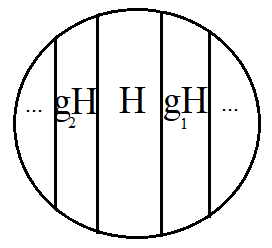
\includegraphics[width=1\linewidth]{Pic1}
		\caption{Седло \\ ($\lambda_1, \lambda_2$ вещественны и разных знаков)}
	\end{minipage}
\end{figure}


\newpage
\subsection*{Задача 5}
\begin{figure}[!h]
	\begin{minipage}[h]{0.49\linewidth}
		\begin{gather*}
			\begin{vmatrix}
				-9 - \lambda & 6\\
				4 & -11 - \lambda
			\end{vmatrix}
			= 
			\lambda^2 + 20\lambda + 75
			=
			\left(\lambda + 5\right)\left(\lambda + 15\right)\\
			\lambda_1 = -5,\ \lambda_2 = -15
		\end{gather*}
		Найдем собственные вектора
		\begin{gather*}
			\lambda_1 = -15\qquad
			A - \lambda_1 I =
			\begin{pmatrix}
				6 & 6\\
				4 & 4
			\end{pmatrix}\\
			v_1 =
			\begin{pmatrix}
				-1 \\ 1
			\end{pmatrix}
		\end{gather*}
		и
		\begin{gather*}
			\lambda_2 = -5\qquad
			A - \lambda_2 I =
			\begin{pmatrix}
				-4 & 6\\
				4 & -6
			\end{pmatrix}\\
			v_2 =
			\begin{pmatrix}
				3 \\ 2
			\end{pmatrix}
		\end{gather*}
		\begin{gather*}
			T = 
			\begin{pmatrix}
				1 & 3\\
				-1 & 2
			\end{pmatrix}\qquad
			T^{-1} = \frac{1}{5}
			\begin{pmatrix}
				2 & -3\\
				1 & 1
			\end{pmatrix}\\
			X = T e^{Jt} T^{-1} = \frac{1}{5} e^{-5t}\\
			\begin{pmatrix}
				1 & 3\\
				-1 & 2
			\end{pmatrix}
			\begin{pmatrix}
				3 & 0\\
				0 & 1
			\end{pmatrix}
			\begin{pmatrix}
				2 & -3\\
				1 & 1
			\end{pmatrix}
			\begin{pmatrix}
				x \\ y
			\end{pmatrix}
		\end{gather*}
	\end{minipage}
	\begin{minipage}[h]{0.49\linewidth}
		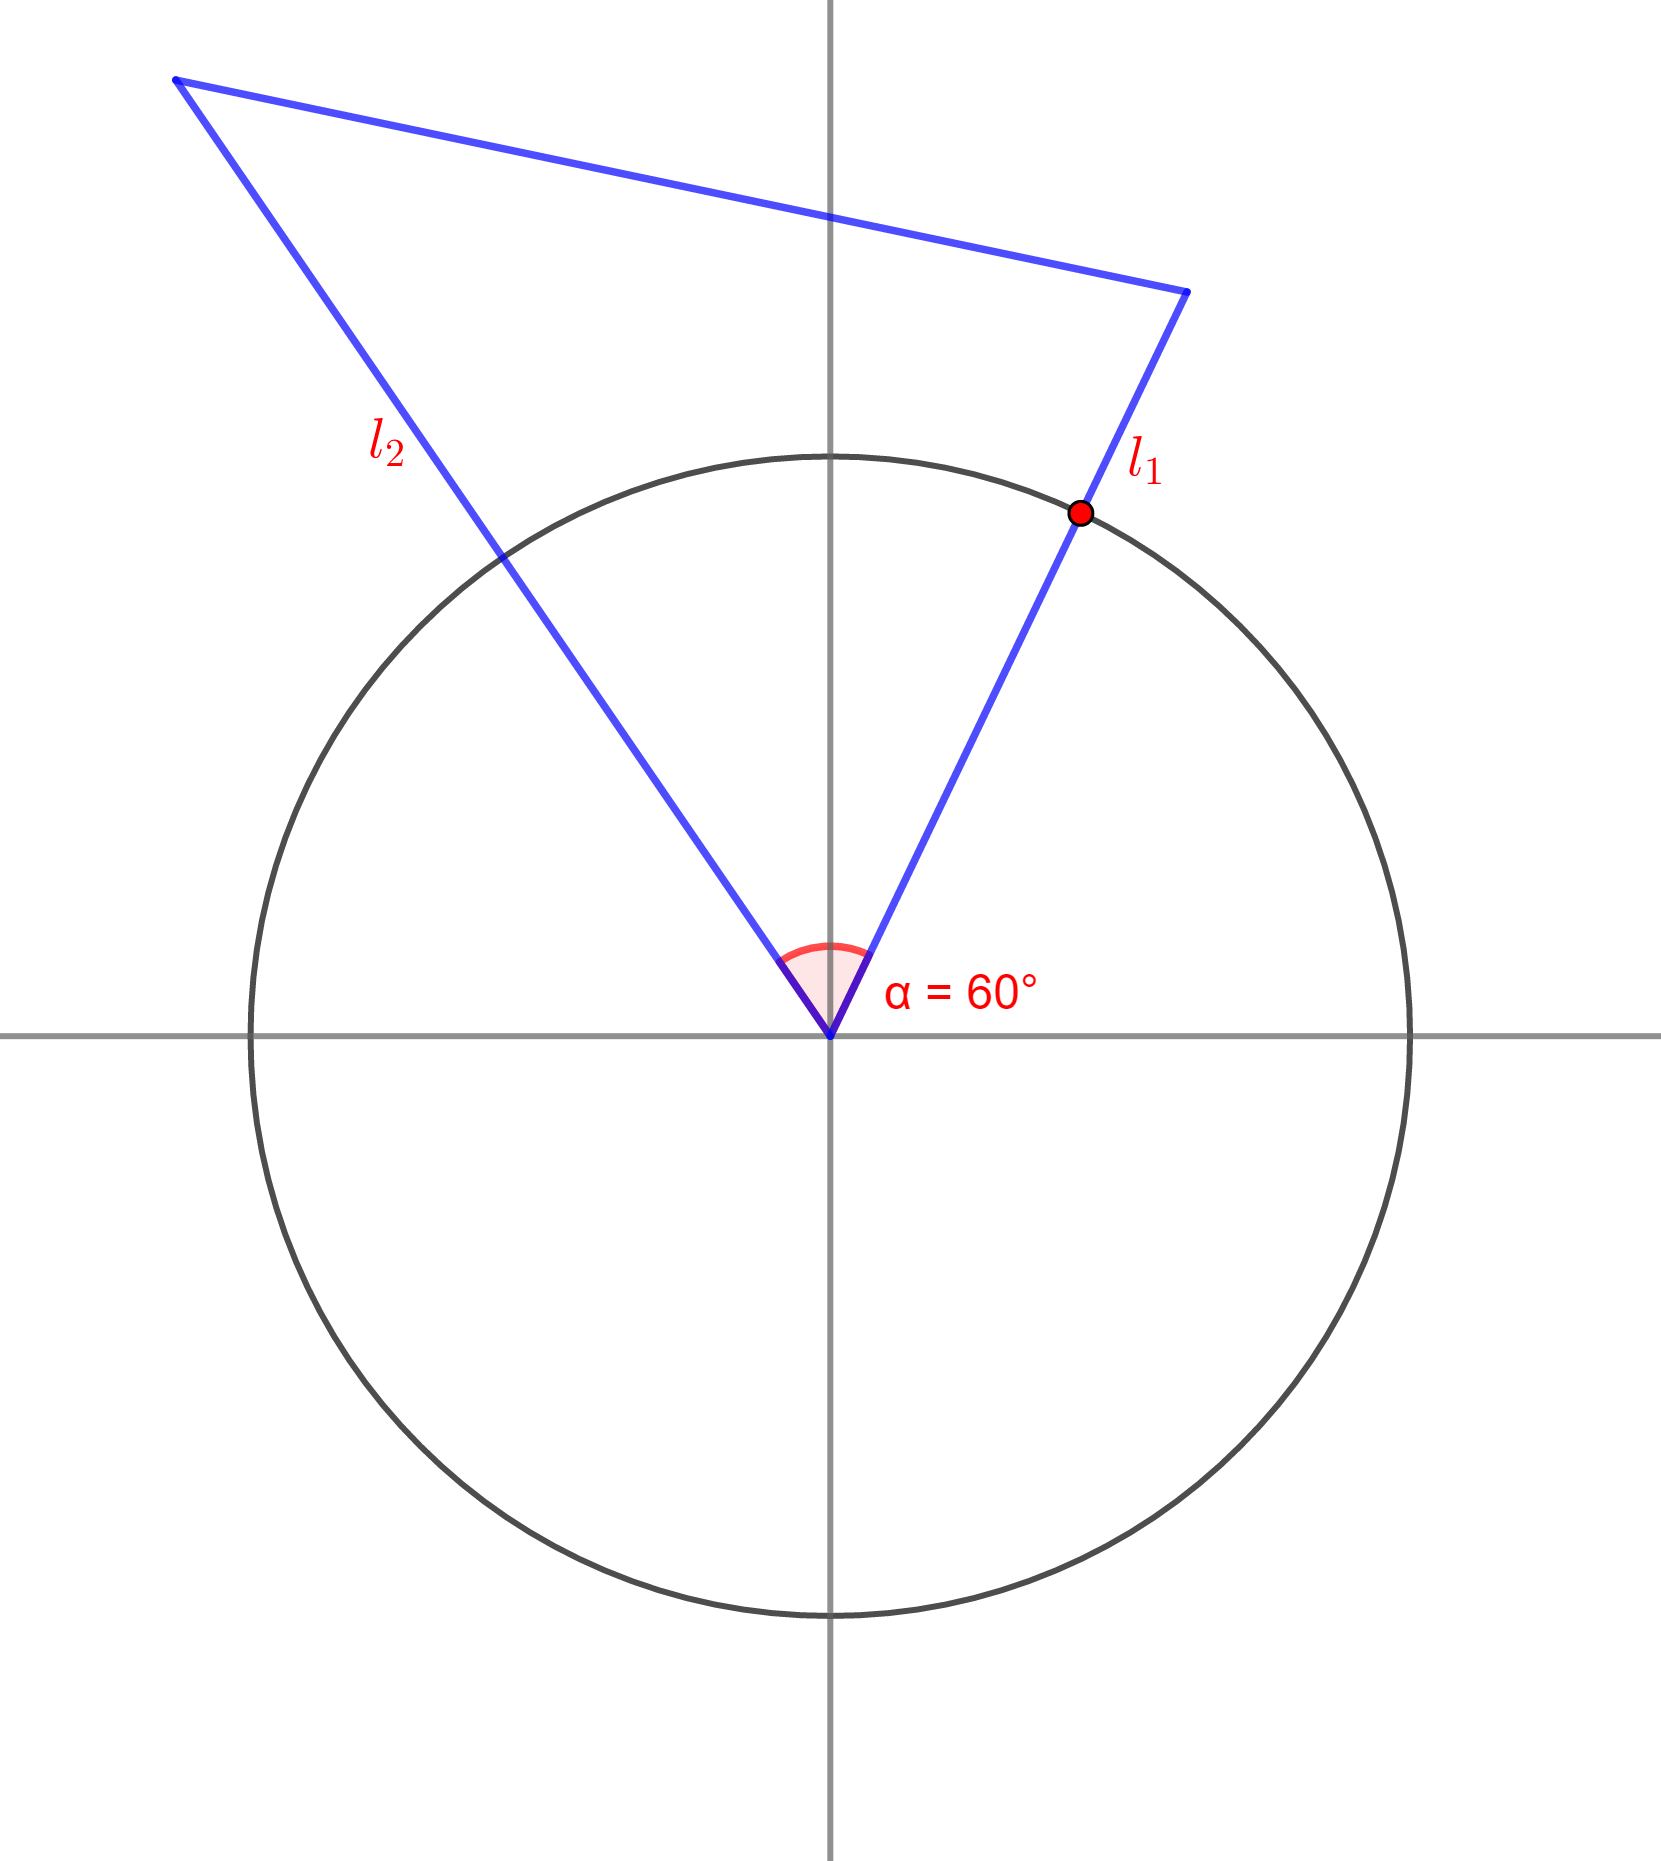
\includegraphics[width=1\linewidth]{Pic2}
		\caption{Устойчивый узел \\ ($\lambda_1, \lambda_2$ вещественны и отрицательны)}
	\end{minipage}
\end{figure}


\newpage
\subsection*{Задача 6}
\begin{figure}[!h]
	\begin{minipage}[h]{0.49\linewidth}
		\begin{gather*}
			\begin{vmatrix}
				-1 - \lambda & 2\\
				-5 & 5 - \lambda
			\end{vmatrix}
			=
			\lambda^2 - 4\lambda + 5\\
			\lambda_1 = 2 - i,\ \lambda_2 = 2 + i\\
			\left(A - \lambda I\right)f = 0\\
			\begin{pmatrix}
				-3-i & 2\\
				-5 & 3-i
			\end{pmatrix}
			\begin{pmatrix}
				2 \\ 3+i
			\end{pmatrix}
			= 0\\
			f = 
			\begin{pmatrix}
				2 \\ 3+i
			\end{pmatrix}\\
			T = ||u,v|| =
			\begin{pmatrix}
				2 & 0\\
				3 & 1
			\end{pmatrix}\qquad
			T^{-1} = \frac{1}{2}
			\begin{pmatrix}
				1 & 0\\
				-3 & 2
			\end{pmatrix}\\
			X\left(t\right) = \frac{1}{2} e^{t}
			\begin{pmatrix}
				2 & 0\\
				3 & 1
			\end{pmatrix}
			\begin{pmatrix}
				\cos t & \sin t\\
				-\sin t & \cos t
			\end{pmatrix}
			\begin{pmatrix}
				1 & 0\\
				-3 & 2
			\end{pmatrix}\\
			v = 
			\begin{pmatrix}
				\dot{x} \\ \dot{y}
			\end{pmatrix}
			|_{x = 0} =
			\begin{pmatrix}
				2 \\ 5
			\end{pmatrix}
			y\\
			\begin{pmatrix}
				\xi \\ \eta
			\end{pmatrix} =
			T^{-1}
			\begin{pmatrix}
				x \\ y
			\end{pmatrix} =
			\frac{1}{2}
			\begin{pmatrix}
				1 & 0\\
				-3 & 2
			\end{pmatrix}
			\begin{pmatrix}
				x \\ y
			\end{pmatrix}\\
			\begin{pmatrix}
				\xi\left(t\right) \\ \eta\left(t\right)
			\end{pmatrix}
			= e^{2t}
			\begin{pmatrix}
				\cos\left(t\right) & \sin\left(t\right)\\
				-\sin\left(t\right) & \cos\left(t\right)
			\end{pmatrix}
			\begin{pmatrix}
				\xi \\ \eta
			\end{pmatrix}
		\end{gather*}
	\end{minipage}
	\begin{minipage}[h]{0.49\linewidth}
		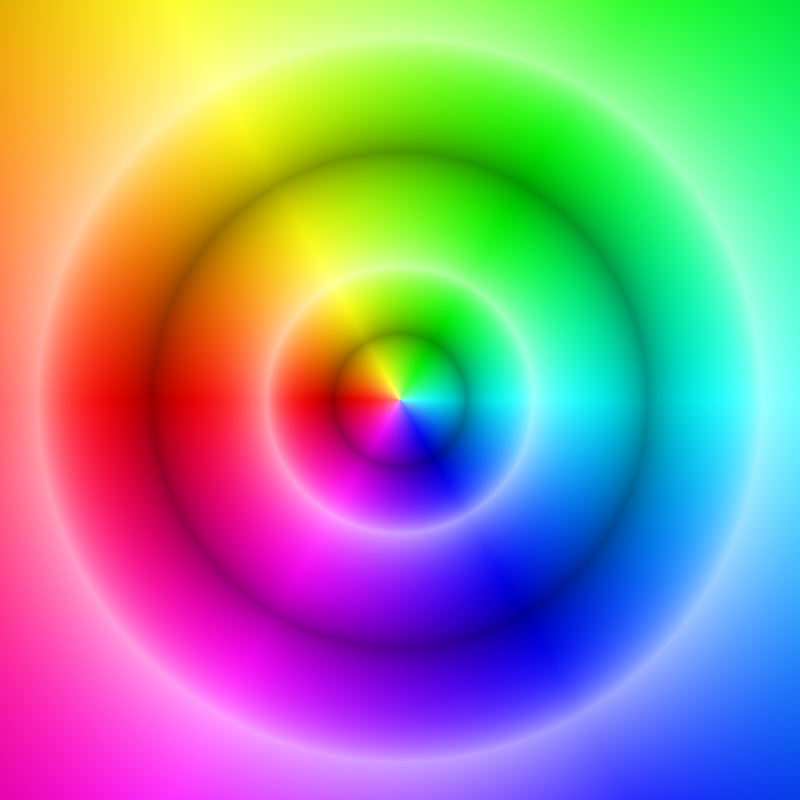
\includegraphics[width=1\linewidth]{Pic3}
		\caption{Неустойчивый фокус \\ ($\lambda_1, \lambda_2$ -- комплексны, $\operatorname{Re}\left(\lambda_{1,2}\right) > 0$)}
	\end{minipage}
\end{figure}


\subsection*{Задача 7}
\begin{figure}[!h]
	\begin{minipage}[h]{0.49\linewidth}
		\begin{gather*}
			\begin{vmatrix}
				\frac{1}{2} - \lambda & -1\\
				1 & -\frac{3}{2} - \lambda
			\end{vmatrix}
			=
			\lambda^2 + \lambda + \frac{1}{4}\\
			\lambda = -\frac{1}{2}
		\end{gather*}
		Найдем собственные вектора
		\begin{gather*}
			\lambda_1 = -\frac{1}{2}\\
			A - \lambda_1 I =
			\begin{pmatrix}
				1 & -1\\
				1 & -1
			\end{pmatrix}\qquad
			v_1 =
			\begin{pmatrix}
				1 \\ 1
			\end{pmatrix}\\
			\left(A + \frac{1}{2}I\right)u_2 = u_1\qquad
			u_2 = 
			\begin{pmatrix}
				1 \\ 0
			\end{pmatrix}\\
			T =
			\begin{pmatrix}
				1 & 1\\
				1 & 0
			\end{pmatrix}\qquad
			T^{-1} =
			\begin{pmatrix}
				0 & 1\\
				1 & -1
			\end{pmatrix}\\
			v = 
			\begin{pmatrix}
				\dot{x} \\ \dot{y}
			\end{pmatrix}
			|_{y = 0}
			=
			\begin{pmatrix}
				1 \\ 2
			\end{pmatrix}x\\
			e^{tJ} = e^{\lambda t}
			\begin{pmatrix}
				1 & t\\
				0 & 1
			\end{pmatrix}\\
			X = T e^{tJ} T^{-1} = e^{-\frac{1}{2} t}
			\begin{pmatrix}
				1 & 1\\
				1 & 0
			\end{pmatrix}
			\begin{pmatrix}
				1 & t\\
				0 & 1
			\end{pmatrix}
			\begin{pmatrix}
				0 & 1\\
				1 & -1
			\end{pmatrix}
			\begin{pmatrix}
				x \\ y
			\end{pmatrix}
		\end{gather*}
	\end{minipage}
	\begin{minipage}[h]{0.49\linewidth}
		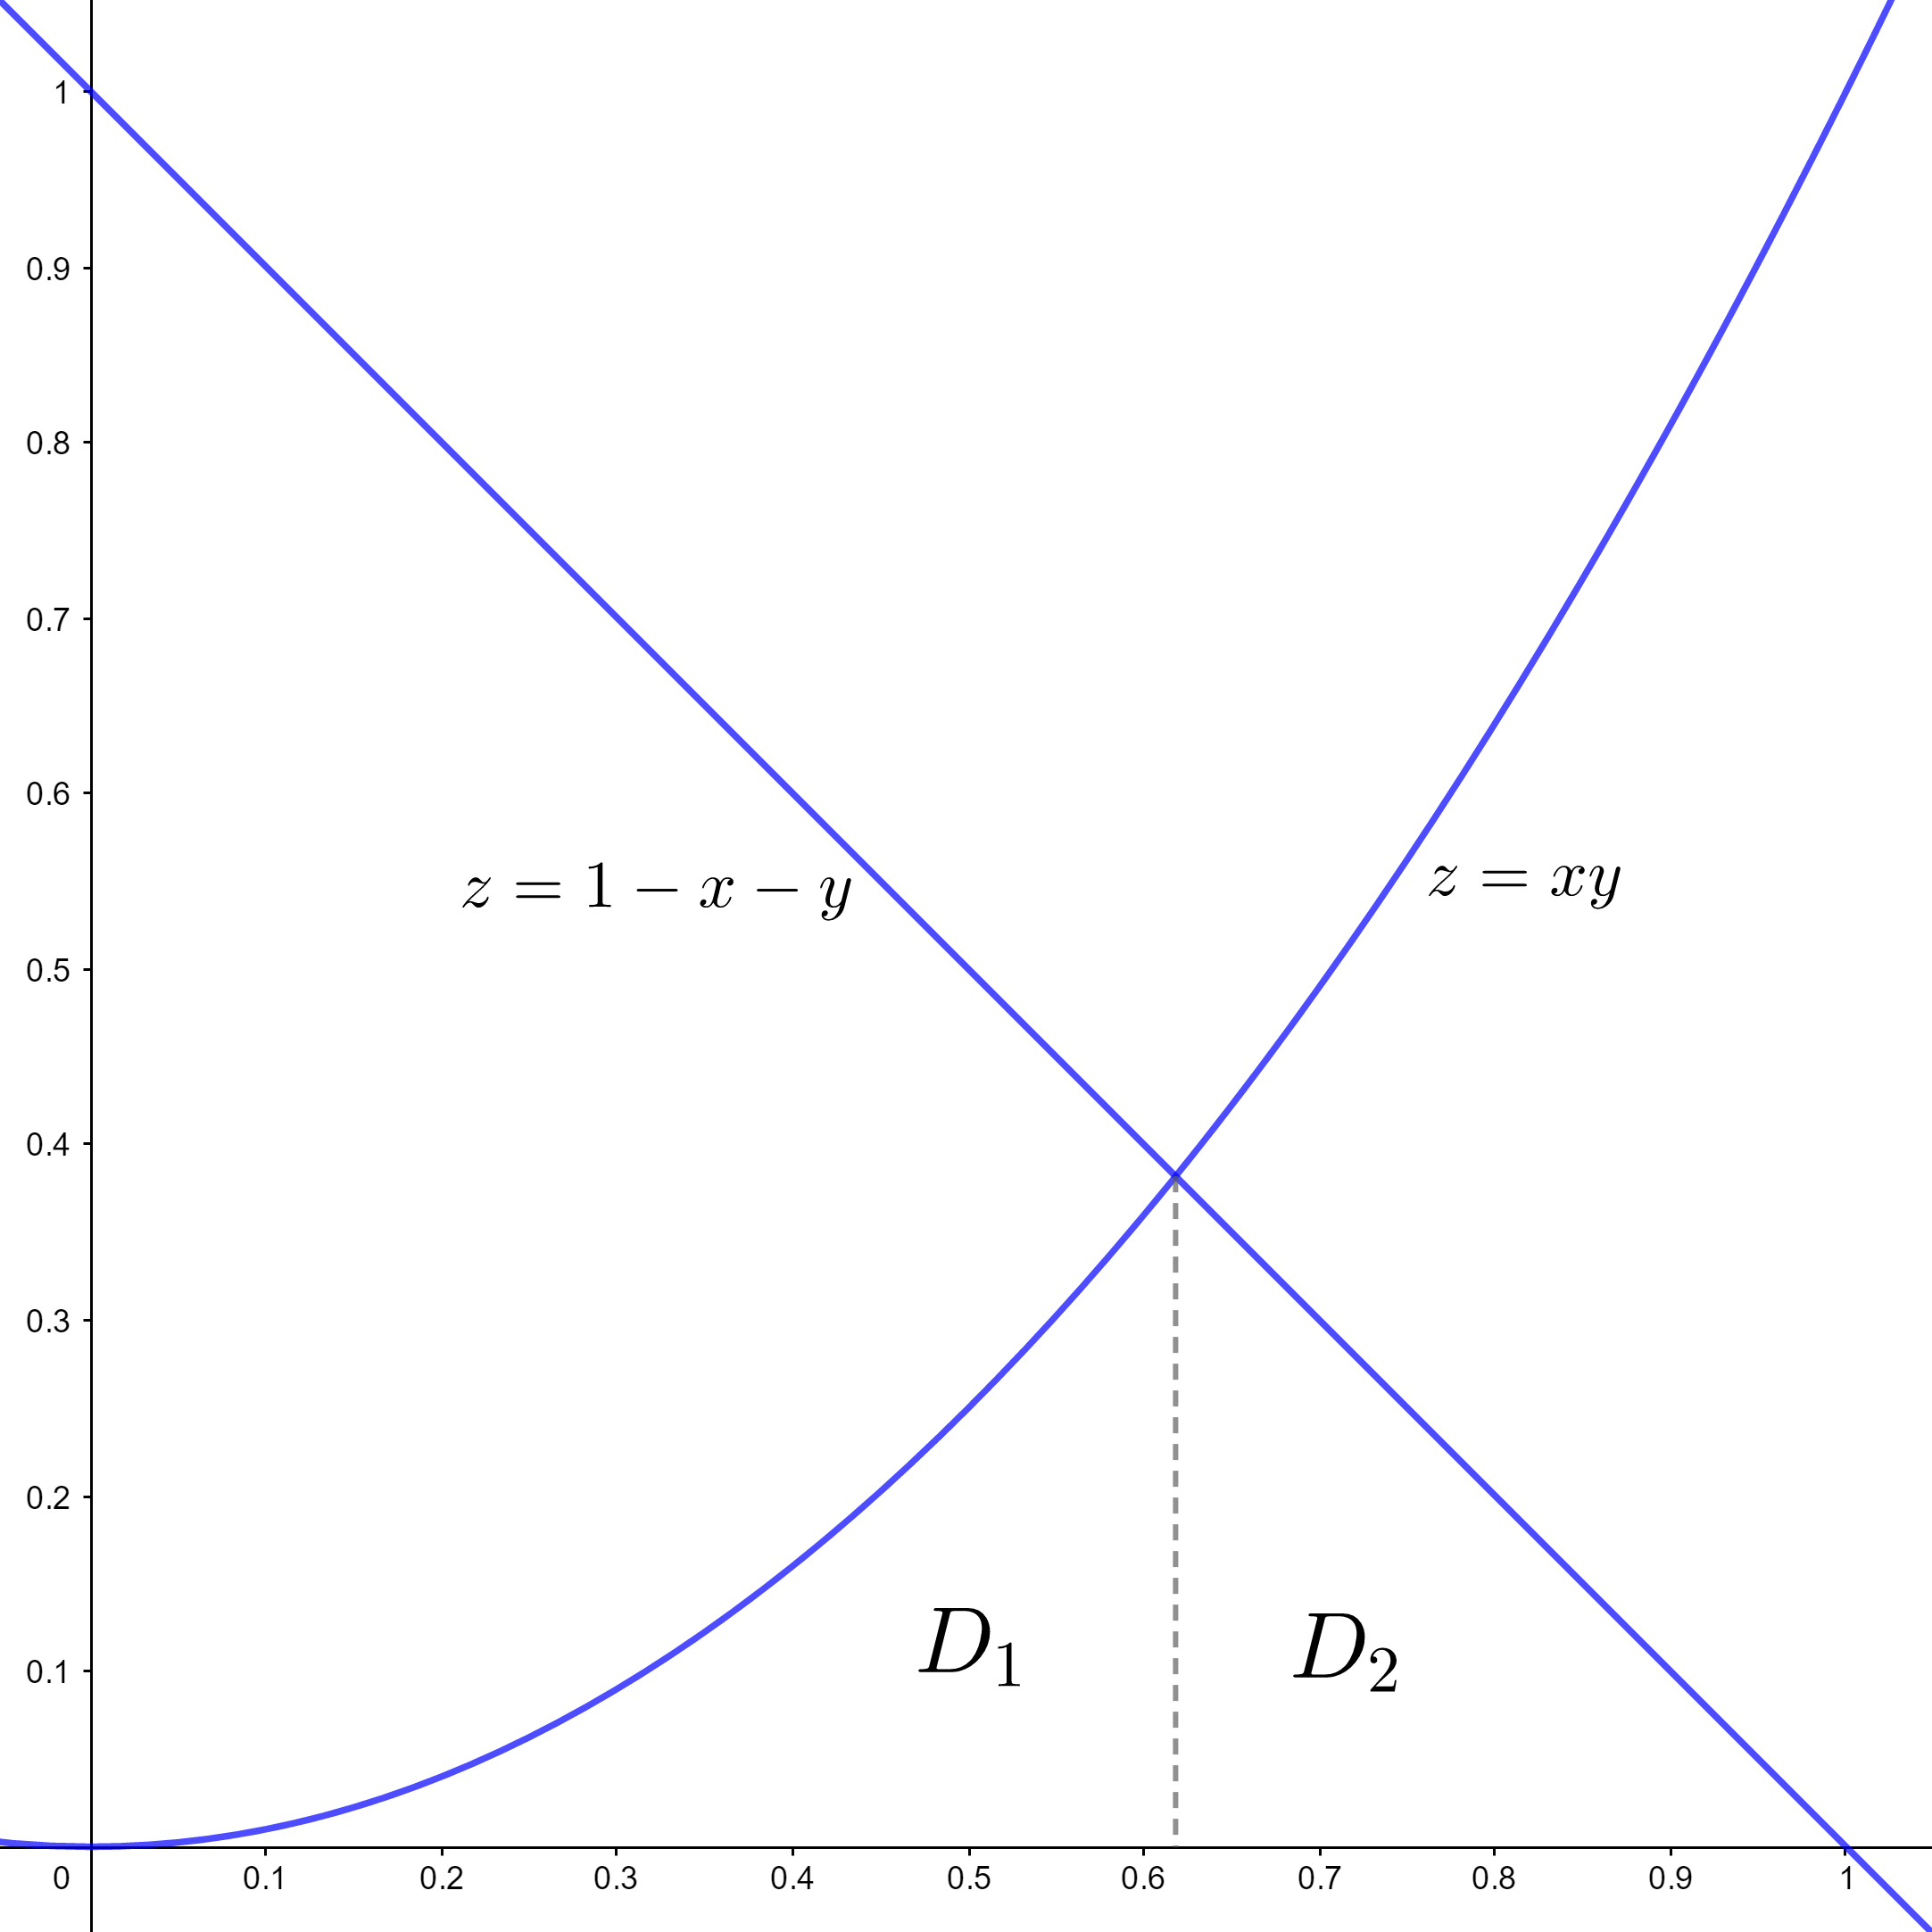
\includegraphics[width=1\linewidth]{Pic4}
		\caption{Вырожденный устойчивый узел}
	\end{minipage}
\end{figure}
\newpage


\newpage
\subsection*{Задача 8}
\begin{figure}[!h]
	\begin{minipage}[h]{0.49\linewidth}
		\begin{gather*}
			\begin{vmatrix}
				13 - \lambda & -20\\
				10 & -15 - \lambda
			\end{vmatrix}
			=
			\lambda^2 + 2\lambda + 5\\
			\lambda_1 = -1-2i,\ \lambda_2 = -1+2i\\
			\left(A - \lambda_1 I\right)f = 0\\
			\begin{pmatrix}
				14 - 2i & -20\\
				10 & -14-2i
			\end{pmatrix}
			\begin{pmatrix}
				v_1^{\left(1\right)} \\ v_2^{\left(1\right)}
			\end{pmatrix}
			= 0\\
			v^{\left(1\right)} =
			\begin{pmatrix}
				7 + i \\ 5
			\end{pmatrix}\\
			T = 
			\begin{pmatrix}
				7 & 1\\
				5 & 0
			\end{pmatrix}\qquad
			T^{-1} = \frac{1}{5}
			\begin{pmatrix}
				0 & -1\\
				-5 & 7
			\end{pmatrix}\\
			\begin{pmatrix}
				\xi\left(t\right) \\ \eta\left(t\right)
			\end{pmatrix}
			= e^{qt}
			\begin{pmatrix}
				\cos wt & \sin wt\\
				-\sin wt & \cos wt
			\end{pmatrix}
			\begin{pmatrix}
				\xi_0 & \eta_0
			\end{pmatrix}\\
			\begin{pmatrix}
				\xi\left(t\right) \\ \eta\left(t\right)
			\end{pmatrix}
			= e^{-t}
			\begin{pmatrix}
				\cos 2t & \sin 2t\\
				-\sin 2t & \cos 2t
			\end{pmatrix}
			\begin{pmatrix}
				\xi_0 & \eta_0
			\end{pmatrix}\\
			v =
			\begin{pmatrix}
				\dot{x} \\ \dot{y}
			\end{pmatrix}
			|_{y = 0} =
			\begin{pmatrix}
				13 \\ 10
			\end{pmatrix}x
		\end{gather*}
	\end{minipage}
	\begin{minipage}[h]{0.49\linewidth}
		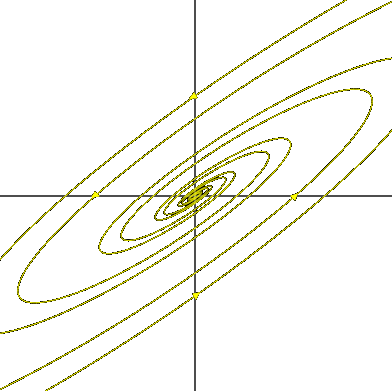
\includegraphics[width=1\linewidth]{Pic5}
		\caption{Устойчивый фокус \\ ($\lambda_1, \lambda_2$ -- комплексны, $\operatorname{Re}\left(\lambda_{1,2}\right) < 0$)}
	\end{minipage}
\end{figure}


\subsection*{Задача 9}
\begin{figure}[!h]
	\begin{minipage}[h]{0.49\linewidth}
		\begin{gather*}
			\begin{vmatrix}
				-1 - \lambda & 2\\
				-1 & 1 - \lambda
			\end{vmatrix}
			=
			\lambda^2 + 1\\
			\lambda_1 = i,\ \lambda_2 = -i\\
			\left(A - iI\right)v_1 = 0\\
			\begin{pmatrix}
				-1-i & 2 \\ -1 & 1-i
			\end{pmatrix}
			\begin{pmatrix}
				x \\ y
			\end{pmatrix}
			= 0\\
			v_1 =
			\begin{pmatrix}
				1-i \\ 1
			\end{pmatrix}
			\begin{pmatrix}
				\xi \\ \eta
			\end{pmatrix}
			=
			T^{-1}
			\begin{pmatrix}
				x \\ y
			\end{pmatrix}\\
			\begin{pmatrix}
				\xi\left(t\right) \\ \eta\left(t\right)
			\end{pmatrix}
			= e^{qt}
			\begin{pmatrix}
				\cos wt & \sin wt \\
				-\sin wt & \cos wt
			\end{pmatrix}
			\begin{pmatrix}
				\xi_0 \\ \eta_0
			\end{pmatrix}\\
			\begin{pmatrix}
				\xi\left(t\right) \\ \eta\left(t\right)
			\end{pmatrix}
			=
			\begin{pmatrix}
				\cos -t & \sin -t \\
				-\sin -t & \cos -t
			\end{pmatrix}
			\begin{pmatrix}
				\xi \\ \eta
			\end{pmatrix}
			= \\ =
			\begin{pmatrix}
				\cos t & -\sin t\\
				\sin t & \cos t
			\end{pmatrix}
			\begin{pmatrix}
				\xi \\ \eta
			\end{pmatrix}\\
			v = 
			\begin{pmatrix}
				\dot{x} \\ \dot{y}
			\end{pmatrix}
			|_{y = 0} =
			\begin{pmatrix}
				-1 \\ -1
			\end{pmatrix}x
		\end{gather*}
	\end{minipage}
	\begin{minipage}[h]{0.49\linewidth}
		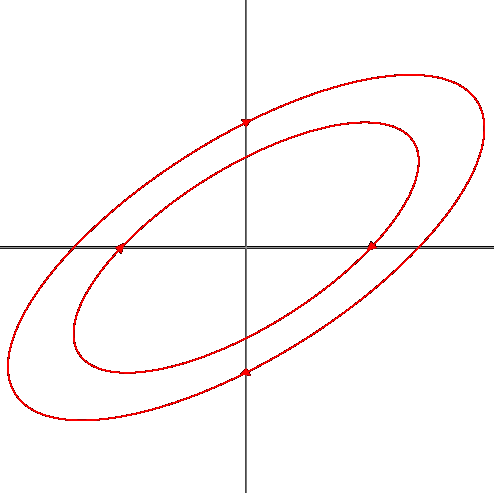
\includegraphics[width=1\linewidth]{Pic6}
		\caption{Центр \\ ($\lambda_1, \lambda_2$ чисто мнимые)}
	\end{minipage}
\end{figure}


\newpage
\subsection*{Задача 10}
\begin{figure}[!h]
	\begin{minipage}[h]{0.49\linewidth}
		\begin{gather*}
			\begin{vmatrix}
				1 - \lambda & 4\\
				-1 & 5 - \lambda
			\end{vmatrix}
			=
			\lambda^2 - 6\lambda + 9
			=
			\left(\lambda - 3\right)^2\\
			\lambda = 3
		\end{gather*}
		Найдем собственные вектора
		\begin{gather*}
			\lambda_1 = 3\\
			A - \lambda_1 I =
			\begin{pmatrix}
				-2 & 4\\
				-1 & 2
			\end{pmatrix}\qquad
			v_1 =
			\begin{pmatrix}
				2 \\ 1
			\end{pmatrix}\\
			\left(A - 3I\right)v_2 = v_1\qquad
			v_2 = 
			\begin{pmatrix}
				1 \\ 1
			\end{pmatrix}\\
			T = 
			\begin{pmatrix}
				2 & 1 \\ 1 & 1
			\end{pmatrix}\qquad
			T^{-1} = \frac{1}{4}
			\begin{pmatrix}
				1 & -1 \\ -1 & 2
			\end{pmatrix}\\
			v =
			\begin{pmatrix}
				\dot{x} \\ \dot{y}
			\end{pmatrix}
			|_{y = 0}
			=
			\begin{pmatrix}
				1 \\ -1
			\end{pmatrix}x\\
			X = T e^{tJ} T^{-1} = e^{3t}
			\begin{pmatrix}
				2 & 1\\
				1 & 1
			\end{pmatrix}
			\begin{pmatrix}
				1 & t\\
				0 & 1
			\end{pmatrix}
			\begin{pmatrix}
				1 & -1\\
				-1 & 2
			\end{pmatrix}
			\begin{pmatrix}
				x \\ y
			\end{pmatrix}
		\end{gather*}
	\end{minipage}
	\begin{minipage}[h]{0.49\linewidth}
		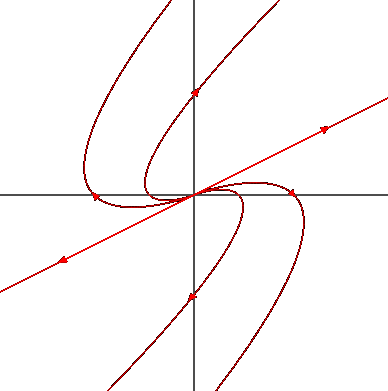
\includegraphics[width=1\linewidth]{Pic7}
		\caption{Вырожденный неустойчивый узел}
	\end{minipage}
\end{figure}